%%%%%%%%%%%%%%%%%%%% author.tex %%%%%%%%%%%%%%%%%%%%%%%%%%%%%%%%%%%
%
% sample root file for your "contribution" to a contributed volume
%
% Use this file as a template for your own input.
%
%%%%%%%%%%%%%%%% Springer %%%%%%%%%%%%%%%%%%%%%%%%%%%%%%%%%%


% RECOMMENDED %%%%%%%%%%%%%%%%%%%%%%%%%%%%%%%%%%%%%%%%%%%%%%%%%%%
\documentclass[graybox]{svmult}

\usepackage[utf8]{inputenc}

% choose options for [] as required from the list
% in the Reference Guide

\usepackage{type1cm}        % activate if the above 3 fonts are
                            % not available on your system
%
\usepackage{makeidx}         % allows index generation
\usepackage{graphicx}        % standard LaTeX graphics tool
                             % when including figure files
\usepackage{multicol}        % used for the two-column index
\usepackage[bottom]{footmisc}% places footnotes at page bottom


\usepackage{newtxtext}       % 
\usepackage{newtxmath}       % selects Times Roman as basic font

\usepackage{algorithm}
\usepackage{algpseudocode}

% see the list of further useful packages
% in the Reference Guide

\makeindex             % used for the subject index
                       % please use the style svind.ist with
                       % your makeindex program

%%%%%%%%%%%%%%%%%%%%%%%%%%%%%%%%%%%%%%%%%%%%%%%%%%%%%%%%%%%%%%%%%%%%%%%%%%%%%%%%%%%%%%%%%

\begin{document}

\title*{Concept Reduction Methods}
% Use \titlerunning{Short Title} for an abbreviated version of
% your contribution title if the original one is too long
\author{Miklós F. Hatwagner}
% Use \authorrunning{Short Title} for an abbreviated version of
% your contribution title if the original one is too long
\institute{Miklós F. Hatwagner \at Széchenyi István University, Győr, Hungary \email{miklos.hatwagner@sze.hu}}
%
% Use the package "url.sty" to avoid
% problems with special characters
% used in your e-mail or web address
%
\maketitle

\abstract*{<To be prepared>}

\abstract{<To be prepared>}

\section{The Motivating Problem}
\label{sec:1}

The title of Adrienn Buruzs's PhD thesis \cite{buruzsphd2015} is ``Evaluation of Sustainable Regional Waste Management Systems with Fuzzy Cognitive Map''. As the title suggests, she analyzed the internal driving forces, dynamic behavior and sustainability of Integrated Waste Management Systems (IWMSs), which are very complex systems including many aspects (environmental, economic, social, institutional, legal and technical) and stakeholders. Even at an early stage of her investigations became apparent that Fuzzy Cognitive Map (FCM) is an appropriate tool to describe the large number of interacting and coupled entities and it copes with the inherent uncertainties of the system.

At first, a new FCM model \cite{buruzs2013developing} was created, which contained six concepts. These concepts were identified on the basis of the literature. The strength of relationships among concepts were defined by the results of a survey filled out by 75 stakeholders. The simulation results provided by FCM were validated later in \cite{buruzs2013advanced}. Time series data were collected based on the relevant literature and it served as the input of a Bacterial Evolutionary Algorithm to learn the connection weights among the already specified concepts and parameter $\lambda$ of the threshold function. The goal of optimization was to find an FCM that generates as similar time series as possible. Unfortunately, a strong contradiction was explored between the models created by experts and machine learning.

In order to resolve the experienced problem the concepts of the original model were decomposed to further 4-7 sub-concepts according to the System-of-Systems approach, which led to a very detailed, completely new model of IWMS \cite{buruzs2013modeling}. A workshop was organized with the help of 12 stakeholders who decided the sub-concepts and their interconnections. The result of their work is a FCM containing 33 concepts in total (Fig.~\ref{fig:flower}). Unfortunately such an extremely complex model is often confusing for the experts (Fig.~\ref{fig:fcmbig}), and to work with them  may be very laborious. Note that the number of connections is a quadratic function of the number of concepts.

That is why, in general, the following approach is suggested to follow in practice: start with an obviously oversized, fine-grained model. Experts are often uncertain about the importance of system components thus it worth include most or all of them in the preliminary model. Then start reducing the model automatically, in an algorithmic way until the balance of model size and required accuracy is found. The numerical accuracy of reduced models are always lower by their nature, but it does not cause a problem in practice until the decisions suggested by them are the same. On the other hand, simpler models are easier to understand, their visual representation is clearer, and it is often more important for experts and managers. In the following sections several possible ways of model reduction is presented.

\begin{figure}[hbt]
  \begin{center}
    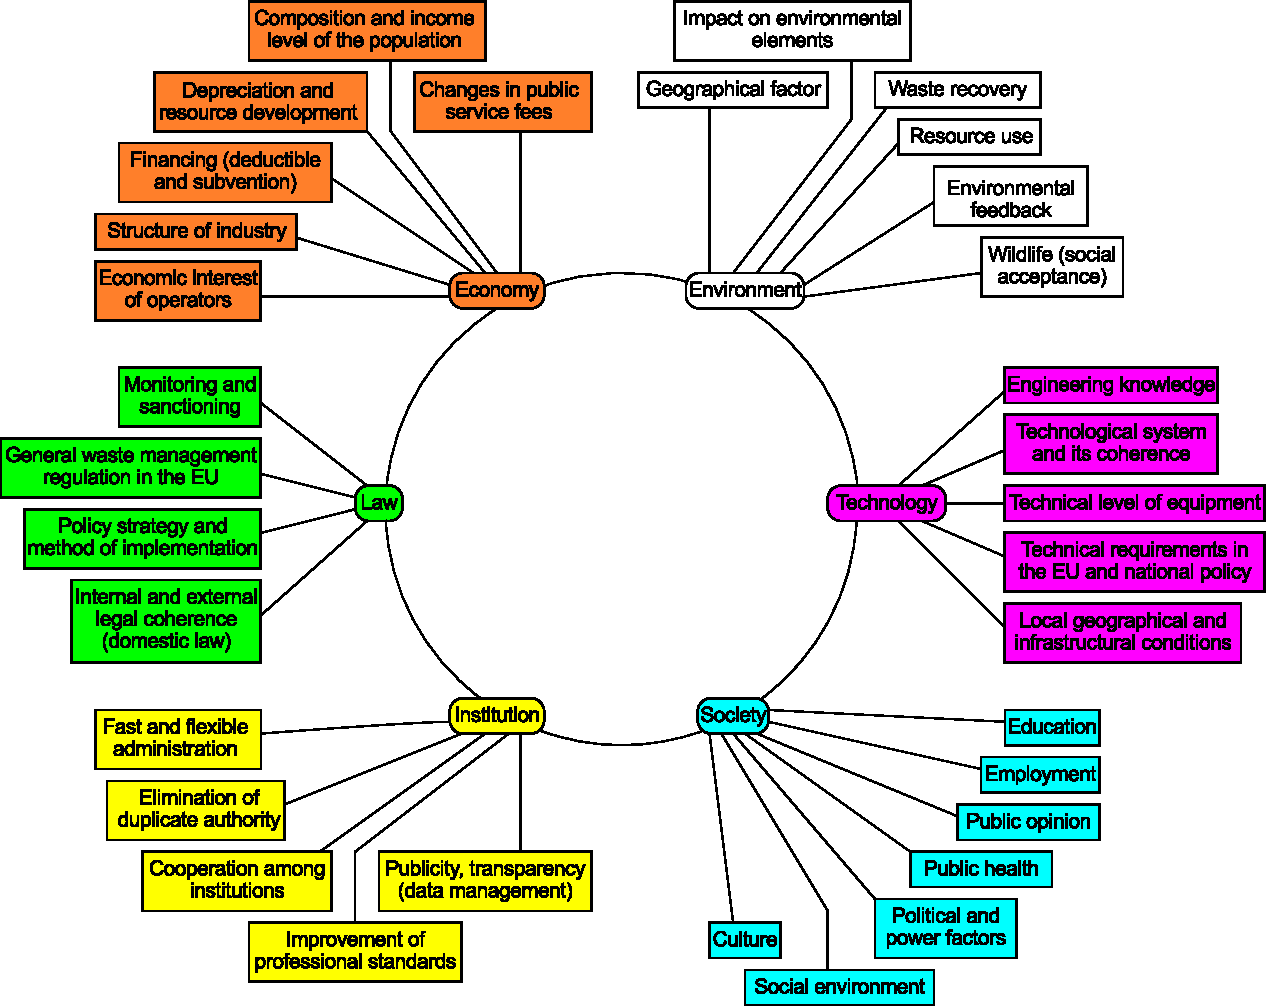
\includegraphics[width=\textwidth]{szines_virag.pdf}
  \end{center}
  \caption{The main concepts and their sub-concepts of regional IWMS.}
  \label{fig:flower}
\end{figure}

\begin{figure}[hbt]
  \begin{center}
    \includegraphics[width=\textwidth]{fcm_big.pdf}
  \end{center}
  \caption{The 33 concept model of regional IWMS and the relationships among its concepts. It is hard to illustrate complex FCM models appropriately and graphical model visualizations often confuse experts.}
  \label{fig:fcmbig}
\end{figure}

\section{Early model reduction methods}
\label{sec:2}

Several methods had been suggested to solve the problem of oversized models before the complex model of IWMS saw the light of the day. These approaches are based on different perspectives.

In \cite{alizadeh2008using} an FCM is learned using historical data and its concepts are grouped into clusters in a unique way. The clustering is based on the DEMATEL \cite{dematel} method. The concepts are arranged on a two dimensional plot. The vertical axis classifies concepts to cause and effect groups, the position of concepts along the horizontal axis expresses the importance of them. Based on this rearrangement of concepts two clustering methods are suggested. The first one uses K-Means clustering to create clusters according to the cause-effect behavior of concepts. The cluster centers replace the original concepts in the reduced model. The second method contains two consecutive steps, and takes also the importance of concepts into consideration. Regardless of the methods applied, experts have to define the number of clusters and they must be disjoint.

FCM was used to predict and discover knowledge about the HIV-1 drug resistance in \cite{NapolesHIV}. The protease protein was modeled by FCM and causalities among sequence positions were estimated by Particle Swarm Optimization. Furthermore, Ant Colony Optimization was also applied in order to find the strongest sequence positions related to the resistance target. After that, some concepts and their connections were removed to decrease the complexity of the model until the quality of inference remained acceptable.

Another reduction method was introduced in \cite{Homenda2014}. Weak concepts and their connections were removed, then the inference capabilities of the simplified model were tested with time series data collected from real-world applications. The reduced model replaced the original if its estimation errors were acceptable.

\section{Fuzzy Tolerance Relations-based reduction methods}
\label{sec:2}

The first results on a novel state reduction method family were presented in \cite{hatwagner2014strategic,hatwagner2015new}. The members of this family differ only in the applied metric, which is used to measure the ``distance'' of concepts from each other. The methods may be considered as generalizations of the state reduction of finite state machines and sequential systems with partially defined states. They are widely applied in digital design where the complexity of the problem makes it possible \cite{kohaviz.jhan.k.2009}. The common idea is to create clusters of identical or similar concepts, and use these clusters instead of their members in the reduced model. The methods are based on Fuzzy Tolerance Relations (FTR), which is an extension of compatibility relations among crisp concepts. The methods examine the connection weights among concepts, because they define the effect on other concepts.

\subsection{Description of the main functions used for reduction}

At the very beginning the new model contains exactly as many clusters as the number of concepts in the original model. These clusters are all disjoint single element sets containing one of the original concepts. In the following, the $i^{th}$ concept is denoted by $C_i$, and similarly, the $i^{th}$ cluster is denoted by $K_i$. The number of concepts is $n$. In the next steps further concepts are added to the clusters if they are ``close enough'' to each member of the cluster. The ``distance'' of concepts can be measured by various metrics. These metrics can be selected according to the specialities of the problem, and they differentiate the members of the algorithm family. Finally, some of these expanded clusters may be identical, containing exactly the same concepts. In order to keep clusters unique, only one of these clusters is retained.

One of the main functions is called $buildCluster$ (Algorithm~\ref{buildCluster}). Its goal is to create a cluster that initially contains only its $initialConcept$. Later this cluster will be expanded by merger of other concepts. The second parameter, $\epsilon$ specifies the maximum allowed distance between current cluster members and the concept under examination. The value of $\epsilon$ must be in the [0,~1] interval. This parameter plays an important role in model reduction, and have to be chosen properly by experts. Low values hardly reduce the size of the model, but high values may cause oversimplification. Its appropriate value is completely problem dependent.

\begin{algorithm}
  \caption{The \emph{buildCluster} function}\label{buildCluster}
  \begin{algorithmic}[1]
    \Function{buildCluster}{$initialConcept,\epsilon$}
    \State $K\gets \{initialConcept\}$
    \For{$i\gets0$; $i<n$; $i++$}
      \If{$i \not= initialConcept$}
        \State $member \gets true$
        \While{$member$ and \Call{hasNextElement}{$K$}}
          \State $j \gets$ \Call{nextElement}{$K$}
          \State $member \gets$ \Call{isNearA}{$j, i, \epsilon$}
        \EndWhile
        \If{$member$}
          \State $K \gets K + \{i\}$
        \EndIf
      \EndIf
    \EndFor
    \State \textbf{return} $c$
    \EndFunction
  \end{algorithmic}
\end{algorithm}

Function $isNearA$ is called several times in $buildCluster$ to decide whether the current concept $C_i$ can become a member of cluster $K$ or not. The number of function calls depends on how many member concepts do the cluster already have. This function (Algorithm~\ref{metricA}) implements one of the possible metrics, but can be repleced by any of the metrics presented here. The last one was suggested in \cite{hatwagnerm.f.koczyl.t.2015}.

\begin{algorithm}
  \caption{Function \emph{isNearA} implementing \emph{Metric ``A''}}\label{metricA}
  \begin{algorithmic}[1]
    \Function{isNearA}{$i, j, \epsilon$}
      \State $near \gets true$
      \For{$k\gets0$; $k<n$ and $near = true$; $k++$}
        \If{$k\not=i$ and $k\not=j$}
          \If{$\frac{|w_{i, k} - w_{j, k}|}{2} \geq \epsilon$ or 
              $\frac{|w_{k, i} - w_{k, j}|}{2} \geq \epsilon$} 
            \State $near \gets false$
          \EndIf
        \EndIf
      \EndFor
      \State \textbf{return} $near$
    \EndFunction
  \end{algorithmic}
\end{algorithm}

Metric ``A'' calculates the absolute difference of two connection weights, $w_{i,k}$ and $w_{j,k}$ from concept $C_i$, a cluster member candidate and concept $C_j$, a concept of cluster $K$ to a third concept $C_k$, where $i \ne j \ne k$, and $i, j, k = 1, ..., n$ and $n$ is the number of concepts. If the half of both this distance and the distance of weights in the opposite direction are below the design variable $\epsilon$ for all $C_k$, $C_i$ is added to cluster $K$.

\begin{algorithm}
  \caption{Function \emph{isNearB} implementing \emph{Metric ``B''}}\label{metricB}
  \begin{algorithmic}[1]
    \Function{isNearB}{$i, j, \epsilon, p$}
      \State $near \gets 0$
      \State $far \gets 0$
      \For{$k\gets0$; $k<n$; $k++$}
        \If{$k\not=i$ and $k\not=j$}
          \If{$\frac{|w_{i, k} - w_{j, k}|}{2} < \epsilon$}
            \State $near \gets near + 1$
          \Else
            \State $far \gets far + 1$
          \EndIf
          \If{$\frac{|w_{k, i} - w_{k, j}|}{2} < \epsilon$}
            \State $near \gets near + 1$
          \Else
            \State $far \gets far + 1$
          \EndIf
        \EndIf
      \EndFor
      \If{$near=0$ or $far/near \geq p$}
        \State \textbf{return} $false$
      \Else
        \State \textbf{return} $true$
      \EndIf
    \EndFunction
  \end{algorithmic}
\end{algorithm}

Metric ``B'' (Algorithm~\ref{metricB}) is a slightly modified version of Metric ``A''. The latter works well in most cases, but sometimes a small proportion of weight differences exceed the allowed value, and prevent the merger of concepts. The second metric provides a simple solution to this problem with the usage of parameter $p$. The metric allows the merger even if the distances are greater than $\epsilon$ in a small, less than $p$ proportion of the investigated cases.

Theoretically the value of $p$ can be any in the $[0, 1]$ interval, but it should be rather low, however. High $p$ values makes possible to practically merge any concepts regardless the value of $\epsilon$, which propably leads to an unusable model.

Metric ``B'' allowed to lower the value of parameter $\epsilon$ with a simple trick, but the third approach (Metric ``C'', Algorithm~\ref{metricC}) allows the omittance of the second parameter $p$ by using the normalized, squared Euclidean distance. It is much easier to tune only one parameter instead of two in practice.

\begin{algorithm}
  \caption{Function \emph{isNearC} implementing \emph{Metric ``C''}}\label{metricC}
  \begin{algorithmic}[1]
    \Function{isNearC}{$i, j, \epsilon$}
      \State $sum \gets 0$
      \For{$k\gets0$; $k<n$; $k++$}
        \If{$k\not=i$ and $k\not=j$}
          \State $sum \gets sum + (w_{i, k} - w_{j, k})^2$
          \State $sum \gets sum + (w_{k, i} - w_{k, j})^2$
        \EndIf
      \EndFor
      \If{$\frac{sum}{(n-2)*8}<\epsilon$}
        \State \textbf{return} $true$
      \Else
        \State \textbf{return} $false$
      \EndIf
    \EndFunction
  \end{algorithmic}
\end{algorithm}

Finally, Metric ``D'' (Algorithm~\ref{metricD}) works with the Manhattan-distance of concepts.

\begin{algorithm}
  \caption{Function \emph{isNearD} implementing \emph{Metric ``D''}}\label{metricD}
  \begin{algorithmic}[1]
    \Function{isNearD}{$i, j, \epsilon$}
      \State $sum \gets 0$
      \For{$k\gets0$; $k<n$; $k++$}
        \If{$k\not=i$ and $k\not=j$}
          \State $sum \gets sum + |w_{i, k} - w_{j, k}|$
          \State $sum \gets sum + |w_{k, i} - w_{k, j}|$
        \EndIf
      \EndFor
      \If{$\frac{sum}{(n-2)*4}<\epsilon$}
        \State \textbf{return} $true$
      \Else
        \State \textbf{return} $false$
      \EndIf
    \EndFunction
  \end{algorithmic}
\end{algorithm}

The applied metrics, its parameters ($\epsilon$, $p$) and also the details of implementation not specified here may affect the result of reduction. For example, if the concepts provided by $nextElement$ are in various orders, the content of clusters may be different, even is the size of the reduced model remains the same. The results should be revised by experts.

The $buildCluster$ function creates one of the clusters of the reduced model. Another function, $buildAllClusters$ (Algorithm~\ref{buildAllClusters}) calls $buildCluster$ subsequently with different $initialConcept$ values. According to the nature of the method, multiple clusters may contain the same concepts. Only one the same clusters will be kept by the algorithm.

\begin{algorithm}
  \caption{The \emph{buildAllClusters} function}\label{buildAllClusters}
  \begin{algorithmic}[1]
    \Function{buildAllClusters}{$\epsilon$}
      \State $clusters \gets \{\}$
      \For{$i\gets0$; $i<n$; $i++$}
        \State $K \gets$ \Call{buildCluster}{$i, \epsilon$}
        \If{!\Call{isElementOf}{$K, clusters$}}
          \State $clusters \gets clusters + \{K\}$
        \EndIf
      \EndFor
      \State \textbf{return} $clusters$
    \EndFunction
  \end{algorithmic}
\end{algorithm}

Function $buildAllClusters$ returns the clusters, the concepts of the reduced model, but the weights among clusters have to be defined also. Function $getWeight$ (Algorithm~\ref{getWeight}) investigates the members of its parameter clusters, $a$ and $b$, and calculates the average (arithmetic mean) weight of relationships between concepts included in cluster $a$ to the concepts of cluster $b$. This function must be called to all possible $a$, $b$ pairs to completely define the reduced model.

\begin{algorithm}
  \caption{The \emph{getWeight} function}\label{getWeight}
  \begin{algorithmic}[1]
    \Function{getWeight}{$a, b$}
      \State $count \gets 0$
      \State $sum \gets 0$
      \While{\Call{hasNextElement}{a}}
        \State $i = \Call{nextElement}{a}$
        \While{\Call{hasNextElement}{b}}
          \State $j = \Call{nextElement}{b}$
          \If{$i\not=j$}
            \State $count \gets count + 1$
            \State $sum \gets sum + w_{i,j}$
          \EndIf
        \EndWhile
      \EndWhile
      \If{$count = 0$}
        \State \textbf{return} $0$
      \Else
        \State \textbf{return} $\frac{sum}{count}$
      \EndIf
    \EndFunction
  \end{algorithmic}
\end{algorithm}

\cite{papageorgiou2017concept} presents step-by-step the reduction 
process of a straightforward, five-concept model in detail.

\subsection{Reduction of the motivating problem}

The original model of the motivating problem (IWMS) contains 33 
concepts and 638 of the theoretically possible 1056 connections, making 
the usage of the model very cumbersome for experts. Several experiments 
were conducted with different metrics and parameter ($\epsilon, p$) 
values. This way the connection between reduction parameters and the 
evoked extent of reduction can be studied. Some interesting results are 
collected in Table~\ref{tab:reductionResults}.

\begin{table}[!t]
\caption{The number of concepts in the reduced connection matrix, using different 
metrics \cite{hatwagnerm.f.koczyl.t.2015}}
\label{tab:reductionResults}
\centering
\begin{tabular}{ccccccccc}
\hline\noalign{\smallskip}
\multicolumn{2}{c}{Metric ``A''} &
  \multicolumn{3}{c}{Metric ``B''} &
  \multicolumn{2}{c}{Metric ``C''} &
  \multicolumn{2}{c}{Metric ``D''} \\
\hline\noalign{\smallskip}
$\epsilon$ & No. of concepts &
  $\epsilon$ & p & No. of concepts &
  $\epsilon$ & No. of concepts &
  $\epsilon$ & No. of concepts \\
\noalign{\smallskip}\svhline\noalign{\smallskip}
0.3 & 28 &
  0.1 & 0.2 & 30 &
  0.01 & 30 &
  0.052 & 32 \\
0.4 & 25 &
  0.2 & 0.05 & 30 &
  0.016 & 28 &
  0.059 & 30 \\
0.5 & 18 &
  0.2 & 0.1 & 26 &
  0.022 & 24 &
  0.078 & 28 \\
0.6 & 15 &
  0.2 & 0.2 & 23 &
  0.027 & 22 &
  0.097 & 26 \\
0.7 & 12 &
  0.3 & 0.05 & 23 &
  0.04 & 20 &
  0.1 & 24 \\
0.8 & 4 &
  0.3 & 0.1 & 21 &
  0.048 & 18 &
  0.104 & 22 \\
\multicolumn{2}{c}{} & 
  0.3 & 0.2 & 15 &
  0.054 & 15 &
  0.149 & 20 \\
\multicolumn{2}{c}{} & 
  0.4 & 0.05 & 19 &
  0.06 & 12 &
  0.173 & 18 \\
\multicolumn{2}{c}{} & 
  0.4 & 0.1 & 10 &
  \multicolumn{2}{c}{} &
  0.188 & 15 \\
\multicolumn{2}{c}{} &
  \multicolumn{3}{c}{} &
  \multicolumn{2}{c}{} &
  0.2 & 13 \\
\noalign{\smallskip}\hline\noalign{\smallskip}
\end{tabular}
\end{table}

Of course, the number of concepts after reduction does not characterize 
the usefulness of the model. 

\subsection{Theoretical background of FTR-based methods}

The name of the reduction methods covered in this section refer to the 
fact that they all based on Fuzzy Tolerance Relations (FTR). If a 
binary relation $R(x,x)$ is \emph{reflexive} and \emph{symmetric}, but 
\emph{not transitive} then it is called a compatibility relation in 
crisp contexts and \emph{tolerance relation} in fuzzy contexts 
\cite{klirg.j.yuanb.1995}. (All further definitions in this subsection 
are also quoted from \cite{klirg.j.yuanb.1995}.) A fuzzy binary 
relation ``$R(x,x)$ is \emph{reflexive} iff $R(x,x) = 1$ for all $x\in 
X$. A fuzzy relation is \emph{symmetric} iff $R(x,y)=R(y,x)$ for all 
$x,y\in X$''. The authors emphasize again that \emph{a FTR is never 
transitive}. (``A fuzzy relation $R(x,x)$ is transitive (\dots) if 
$R(x,z)\geq \max_{y\in Y}\min[R(x,y), R(y,z)]$ is satisfied for each 
pair $\langle x,z\rangle\in X^2$.'')

The four metrics defined by \emph{isNear} functions are all real 
distance functions. As such, the following conditions are satisfied by 
function $d$, where $d:R(X,X)\rightarrow \mathbb{R}, \forall x,y,z \in 
X$:

\begin{enumerate}
\item $d(x,x) \geq 0$
\item $d(x,y) = 0$ iff $x=y$
\item $d(x,y) = d(y,x)$ (symmetry)
\item $d(x,z) \leq d(x,y) + d(y,z)$ (triangle inequality)
\end{enumerate}

The applied metrics are symmetric functions, and \emph{isNear} 
functions always return true ($R(x,x) = 1$ or $\mu = 1$) if values of 
the parameters are the same (reflexivity). These metrics generate 
non-transitive mergers, therefore they create FTRs.

Function \emph{buildAllClusters} initiates the process of cluster 
building with every single concepts as \emph{initialConcept}. The called 
\emph{buildCluster} function may extend these initially single element 
clusters with other concepts according to the connection weights among 
concepts and the value of parameter $\epsilon$. According to this 
behavior, the following properties hold:

\begin{itemize}
  \item all concepts of the original model will be included in at least one cluster, 
  \item the same concept may be included in multiple clusters, thus 
  clusters overlap (Fig.~\ref{fig:overlapping}).
\end{itemize}

\begin{figure}[hbt]
  \sidecaption
  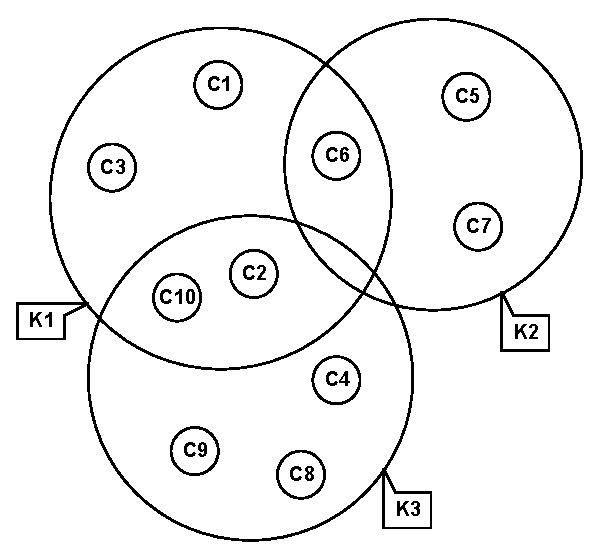
\includegraphics[width=7cm]{clusters.eps}
  \caption{Basic example of overlapping clusters \cite{hatwagnerm.f.koczyl.t.2015}}
  \label{fig:overlapping}
\end{figure}

\subsection{Two-Staged Learning Based Reduction}

Original and reduced models obviously behave in a different way 
because the latter have less concepts, the concepts 
represent different objects of the real system, and the weights of 
relationships among concepts must be different as well. The extent 
of differences rely primarily on the design parameter $\epsilon$ of 
model reduction. Certain differences in model behaviors do not mean 
a problem until the same decisions can be made with both models. 
Unfortunately behavioral differences are hard to measure, because 
the values of concepts representing different objects cannot be 
compared to each other. In order to overcome this difficulty the 
following three groups of concepts were distingiuished in \cite
{hatwagner2018two}: 
\begin{enumerate}
  \item Concepts affecting other concepts but not affected by other 
  concepts are called \emph{input concepts}. They serve as the inputs 
  of the modeled system. The states of these concepts remain the same 
  during simulations, thus they neither need transformation function 
  nor its parameter $\lambda$.
  \item Some concepts are both affected by other concepts and they 
  also have an effect on more or less concepts. These are the 
  \emph{intermediate concepts}.
  \item The third group of concepts is the \emph{output 
  concepts} (or decision concepts). Their states are defined by 
  other concepts, but they do not influence the state of any other 
  concepts. 
\end{enumerate}
In order to make the behavioral difference of original and reduced 
models measurable, a modified reduction method was suggested in 
\cite{hatwagner2018two}, that allows the merger of intermediate 
concepts only. This way simulations can be started with the same 
initial input concept states and the results in output concepts can 
be directly compared. The relation between the value of design 
parameter $\epsilon$ and simulation error of the reduced model can be 
defined statistically using several models, many initial state vectors 
and $\epsilon$ values.

The \emph{getWeight} function was also revised. The original version of 
it (\emph{average}, Algorithm~\ref{getWeight}) defines the weight of connection 
between two clusters ($a$ and $b$) as the arithmetic mean (average) weight of 
connections between concepts included in the corresponding clusters. 
More formally, the weight calculation can be expressed by Eq.~\ref
{eq:getWeight-average}.

\begin{equation}
  \label{eq:getWeight-average}
  w_a(a,b) = \frac{\sum_{i \in a} \sum_{j \in b} a(i,j) \times w_{ij}}{\sum_{i \in a} \sum_{j \in b} a(i,j)}
\end{equation}

\noindent where $a(i,j)$ is defined as

\begin{equation}
  \label{eq:isConnection}
  a(i,j) = \left\{ \begin{array}{ll} 
                     1 & \textrm{if } w_{ij} \neq 0 \textrm{,} \\
                     0 & \textrm{otherwise.}
                   \end{array} \right.
\end{equation}

The second approach (\emph{weighted average}) calculates the weighted 
average of connection weights among cluster members. Greater 
inter-concept weights play more important role in the definition of 
inter-cluster weights (see Eq.~\ref{eq:getWeight-weightedAverage}).

\begin{equation}
  \label{eq:getWeight-weightedAverage}
  w_w(a,b) = \frac{\sum_{i \in a} \sum_{j \in b} a(i,j) \times |w_{ij}| \times w_{ij}}{\sum_{i \in a} \sum_{j \in b} a(i,j) 
\times |w_{ij}|}
\end{equation}

The third method (\emph{extreme}, Eq.~\ref{eq:getWeight-extreme}) selects 
the connection between clusters with the maximum absolute value, and 
that will be used between the clusters. If there are conncections 
with the same absolute value but different sign, the positive one 
will be chosen.

\begin{equation}
  \label{eq:getWeight-extreme}
  w_e(a,b) = \left\{ \begin{array}{ll}
                       min(w_{ij}) & \textrm{if } \left| min(w_{ij}) \right| > \left| max(w_{ij}) \right| \\
                       & \textrm{for } \forall i \in a \wedge \forall j \in b \textrm{,} \\
                       max(w_{ij}) & \textrm{otherwise.}
                     \end{array} \right.
\end{equation}

The last method (\emph{sum}, Eq.~\ref{eq:getWeight-sum}) adds up the 
weight of connections among clusters. If that would not fit in the 
allowed $[-1,~+1]$ interval, the method rounds the weight up or 
down to the nearest allowed value.

\begin{equation}
  \label{eq:getWeight-sum}
  w_s(a,b) = \left\{ \begin{array}{ll}
                       1 & \textrm{if } s(a,b) > 1 \\
                       -1 & \textrm{if } s(a,b) < -1 \\
                       s(a,b) & \textrm{otherwise.}
                     \end{array} \right.
\end{equation}

where $s(a,b)$ is calculated as

\begin{equation}
  \label{eq:sum}
  s(a,b) = \sum_{i \in a} \sum_{j \in b} w_{ij}
\end{equation}

Model reduction inevitably causes information loss and reduced 
models behave less reliable. In order to somewhat compensate this 
problem, concepts of the reduced model did not share a common 
$\lambda$ as in the original model but used different steepness 
parameters. Their values were identified by an evolutionary 
optimization method, the Big Bang -- Big Crunch (BB-BC) \cite
{yesilenginurbasleon2010} algorithm. The relatively low 
computational cost and high convergence speed made it a proper choice, 
moreover, the designer have to set only a few parameters to work 
with it. Input concepts have constant states during simulation, thus 
they do not need parameter $\lambda$ at all. Every output concept 
had its own $\lambda_{oj}$ parameter. It would have been the best if 
every intermediate concept has its own $\lambda$ value, but it 
would have increased the computational cost of the optimization 
disproportionately. As a trade-off, every intermediate concepts had a 
common $\lambda_{i}$ parameter. According to these changes, the 
inference formula was modified to Eq.~\ref{eq:manyLambdaThreshold}:

\begin{equation}
  \label{eq:manyLambdaThreshold}
  A_i^{(t+1)} = f_i\left(\sum_{j=1}^{M} w_{ji}A_j^{(t)} + A_i^{(t)}\right), i \neq j
\end{equation}

where $f_i$ is a sigmoidal threshold function, and its slope is 
specified by $\lambda_i$. These parameters were identified by the 
BB-BC algorithm that minimized the objective function given by Eq.~
\ref{eq:objective}:

\begin{equation}
  \label{eq:objective}
  \sum_{i=1}^{m} a(s_i) \times \sum_{j=1}^{n} |o_{ij} - r_{ij}|
\end{equation}


\begin{acknowledgement}
If you want to include acknowledgments of assistance and the like at 
the end of an individual chapter please use the \verb|acknowledgement| 
environment -- it will automatically be rendered in line with the preferred layout.
\end{acknowledgement}

%%%%%%%%%%%%%%%%%%%%%%%% referenc.tex %%%%%%%%%%%%%%%%%%%%%%%%%%%%%%
% sample references
% %
% Use this file as a template for your own input.
%
%%%%%%%%%%%%%%%%%%%%%%%% Springer-Verlag %%%%%%%%%%%%%%%%%%%%%%%%%%
%
% BibTeX users please use
\bibliographystyle{plain}
\bibliography{../hfmbibfile}
%
%\biblstarthook{References may be \textit{cited} in the text either by number (preferred) or by author/year.\footnote{Make sure that all references from the list are cited in the text. Those not cited should be moved to a separate \textit{Further Reading} section or chapter.} If the citatiion in the text is numbered, the reference list should be arranged in ascending order. If the citation in the text is author/year, the reference list should be \textit{sorted} alphabetically and if there are several works by the same author, the following order should be used:
%\begin{enumerate}
%\item all works by the author alone, ordered chronologically by year of publication
%\item all works by the author with a coauthor, ordered alphabetically by coauthor
%\item all works by the author with several coauthors, ordered chronologically by year of publication.
%\end{enumerate}
%The \textit{styling} of references\footnote{Always use the standard abbreviation of a journal's name according to the ISSN \textit{List of Title Word Abbreviations}, see \url{http://www.issn.org/en/node/344}} depends on the subject of your book:
%\begin{itemize}
%\item The \textit{two} recommended styles for references in books on \textit{mathematical, physical, statistical and computer sciences} are depicted in ~\cite{science-contrib, science-online, science-mono, science-journal, science-DOI} and ~\cite{phys-online, phys-mono, phys-journal, phys-DOI, phys-contrib}.
%\item Examples of the most commonly used reference style in books on \textit{Psychology, Social Sciences} are~\cite{psysoc-mono, psysoc-online,psysoc-journal, psysoc-contrib, psysoc-DOI}.
%\item Examples for references in books on \textit{Humanities, Linguistics, Philosophy} are~\cite{humlinphil-journal, humlinphil-contrib, humlinphil-mono, humlinphil-online, humlinphil-DOI}.
%\item Examples of the basic Springer Nature style used in publications on a wide range of subjects such as \textit{Computer Science, Economics, Engineering, Geosciences, Life Sciences, Medicine, Biomedicine} are ~\cite{basic-contrib, basic-online, basic-journal, basic-DOI, basic-mono}. 
%\end{itemize}
%}

%\begin{thebibliography}{99.}%
%% and use \bibitem to create references.
%%
%% Use the following syntax and markup for your references if 
%% the subject of your book is from the field 
%% "Mathematics, Physics, Statistics, Computer Science"
%%
%% Contribution 
%\bibitem{science-contrib} Broy, M.: Software engineering --- from auxiliary to key technologies. In: Broy, M., Dener, E. (eds.) Software Pioneers, pp. 10-13. Springer, Heidelberg (2002)
%%
%% Online Document
%\bibitem{science-online} Dod, J.: Effective substances. In: The Dictionary of Substances and Their Effects. Royal Society of Chemistry (1999) Available via DIALOG. \\
%\url{http://www.rsc.org/dose/title of subordinate document. Cited 15 Jan 1999}
%%
%% Monograph
%\bibitem{science-mono} Geddes, K.O., Czapor, S.R., Labahn, G.: Algorithms for Computer Algebra. Kluwer, Boston (1992) 
%%
%% Journal article
%\bibitem{science-journal} Hamburger, C.: Quasimonotonicity, regularity and duality for nonlinear systems of partial differential equations. Ann. Mat. Pura. Appl. \textbf{169}, 321--354 (1995)
%%
%% Journal article by DOI
%\bibitem{science-DOI} Slifka, M.K., Whitton, J.L.: Clinical implications of dysregulated cytokine production. J. Mol. Med. (2000) doi: 10.1007/s001090000086 
%%
%\bigskip

%% Use the following (APS) syntax and markup for your references if 
%% the subject of your book is from the field 
%% "Mathematics, Physics, Statistics, Computer Science"
%%
%% Online Document
%\bibitem{phys-online} J. Dod, in \textit{The Dictionary of Substances and Their Effects}, Royal Society of Chemistry. (Available via DIALOG, 1999), 
%\url{http://www.rsc.org/dose/title of subordinate document. Cited 15 Jan 1999}
%%
%% Monograph
%\bibitem{phys-mono} H. Ibach, H. L\"uth, \textit{Solid-State Physics}, 2nd edn. (Springer, New York, 1996), pp. 45-56 
%%
%% Journal article
%\bibitem{phys-journal} S. Preuss, A. Demchuk Jr., M. Stuke, Appl. Phys. A \textbf{61}
%%
%% Journal article by DOI
%\bibitem{phys-DOI} M.K. Slifka, J.L. Whitton, J. Mol. Med., doi: 10.1007/s001090000086
%%
%% Contribution 
%\bibitem{phys-contrib} S.E. Smith, in \textit{Neuromuscular Junction}, ed. by E. Zaimis. Handbook of Experimental Pharmacology, vol 42 (Springer, Heidelberg, 1976), p. 593
%%
%\bigskip
%%
%% Use the following syntax and markup for your references if 
%% the subject of your book is from the field 
%% "Psychology, Social Sciences"
%%
%%
%% Monograph
%\bibitem{psysoc-mono} Calfee, R.~C., \& Valencia, R.~R. (1991). \textit{APA guide to preparing manuscripts for journal publication.} Washington, DC: American Psychological Association.
%%
%% Online Document
%\bibitem{psysoc-online} Dod, J. (1999). Effective substances. In: The dictionary of substances and their effects. Royal Society of Chemistry. Available via DIALOG. \\
%\url{http://www.rsc.org/dose/Effective substances.} Cited 15 Jan 1999.
%%
%% Journal article
%\bibitem{psysoc-journal} Harris, M., Karper, E., Stacks, G., Hoffman, D., DeNiro, R., Cruz, P., et al. (2001). Writing labs and the Hollywood connection. \textit{J Film} Writing, 44(3), 213--245.
%%
%% Contribution 
%\bibitem{psysoc-contrib} O'Neil, J.~M., \& Egan, J. (1992). Men's and women's gender role journeys: Metaphor for healing, transition, and transformation. In B.~R. Wainrig (Ed.), \textit{Gender issues across the life cycle} (pp. 107--123). New York: Springer.
%%
%% Journal article by DOI
%\bibitem{psysoc-DOI}Kreger, M., Brindis, C.D., Manuel, D.M., Sassoubre, L. (2007). Lessons learned in systems change initiatives: benchmarks and indicators. \textit{American Journal of Community Psychology}, doi: 10.1007/s10464-007-9108-14.
%%
%%
%% Use the following syntax and markup for your references if 
%% the subject of your book is from the field 
%% "Humanities, Linguistics, Philosophy"
%%
%\bigskip
%%
%% Journal article
%\bibitem{humlinphil-journal} Alber John, Daniel C. O'Connell, and Sabine Kowal. 2002. Personal perspective in TV interviews. \textit{Pragmatics} 12:257--271
%%
%% Contribution 
%\bibitem{humlinphil-contrib} Cameron, Deborah. 1997. Theoretical debates in feminist linguistics: Questions of sex and gender. In \textit{Gender and discourse}, ed. Ruth Wodak, 99--119. London: Sage Publications.
%%
%% Monograph
%\bibitem{humlinphil-mono} Cameron, Deborah. 1985. \textit{Feminism and linguistic theory.} New York: St. Martin's Press.
%%
%% Online Document
%\bibitem{humlinphil-online} Dod, Jake. 1999. Effective substances. In: The dictionary of substances and their effects. Royal Society of Chemistry. Available via DIALOG. \\
%http://www.rsc.org/dose/title of subordinate document. Cited 15 Jan 1999
%%
%% Journal article by DOI
%\bibitem{humlinphil-DOI} Suleiman, Camelia, Daniel C. O'Connell, and Sabine Kowal. 2002. `If you and I, if we, in this later day, lose that sacred fire...': Perspective in political interviews. \textit{Journal of Psycholinguistic Research}. doi: 10.1023/A:1015592129296.
%%
%%
%%
%\bigskip
%%
%%
%% Use the following syntax and markup for your references if 
%% the subject of your book is from the field 
%% "Computer Science, Economics, Engineering, Geosciences, Life Sciences"
%%
%%
%% Contribution 
%\bibitem{basic-contrib} Brown B, Aaron M (2001) The politics of nature. In: Smith J (ed) The rise of modern genomics, 3rd edn. Wiley, New York 
%%
%% Online Document
%\bibitem{basic-online} Dod J (1999) Effective Substances. In: The dictionary of substances and their effects. Royal Society of Chemistry. Available via DIALOG. \\
%\url{http://www.rsc.org/dose/title of subordinate document. Cited 15 Jan 1999}
%%
%% Journal article by DOI
%\bibitem{basic-DOI} Slifka MK, Whitton JL (2000) Clinical implications of dysregulated cytokine production. J Mol Med, doi: 10.1007/s001090000086
%%
%% Journal article
%\bibitem{basic-journal} Smith J, Jones M Jr, Houghton L et al (1999) Future of health insurance. N Engl J Med 965:325--329
%%
%% Monograph
%\bibitem{basic-mono} South J, Blass B (2001) The future of modern genomics. Blackwell, London 
%%
%\end{thebibliography}

\end{document}
